\documentclass[pdftex,letterpaper,11pt]{article}
\usepackage[top=1in,bottom=1in,left=1in,right=1in]{geometry}

\usepackage[dvips]{graphicx}
\usepackage{amsmath}
\usepackage{amssymb}
\usepackage{color}
\usepackage[yyyymmdd]{datetime}
\usepackage{fancyhdr}
\usepackage{fancyvrb}
\usepackage[hidelinks]{hyperref}
\usepackage{pslatex}

\usepackage{subfig}
\usepackage{graphicx}
\usepackage[cache=false]{minted}

\usepackage{fancyhdr}
\usepackage{poemscol}
\usepackage{lmodern}

\pagestyle{fancy}

\title{%
	It is the Champion \\
	\large Prototype findings}

\author{Jordan Aceto}

\setlength{\parindent}{0mm}
\setlength{\parskip}{3mm}

\lfoot{Jordan Aceto}
\cfoot{Page \thepage}
\rfoot{PDF: \today, \currenttime}

\renewcommand{\footrulewidth}{0.4pt}

\begin{document}

\maketitle

\tableofcontents

\newpage

\section{Basic Features}

\begin{itemize}
\item Made of mostly ``junk box'' parts.
\item Single ended 6550 ouput stage, cathode biased.
\item Two 12AX7 tubes in the preamp.
\item Fairly high gain ``Trainwreck-ish'' preamp with four gain stages.
\item Conventional treble, middle, bass tone stack.
\item Gain and master volume controls.
\item Point to point wiring in a gutted Fender Vibro-Champ XD cabinet.
\item Power transformer: Hammond 276x.
\item Output transformer: Edcor GXSE15-8-3.5k
\item DC filaments for the first 12AX7, supplied by a separate Antek AN-0115 transformer.
\end{itemize}

\newpage

\section{Preamp}

The preamp is fairly similar to the ``Trainwreck'' circuit. It has the plate driven tone stack early on in the signal path, followed by a gain stage, and then a cold-clipper stage. Since this is a single ended amp without a phase inverter, an additional gain stage is used before the master volume for some extra crunch.

I tweaked some of the values in the tone stack, and added a treble-cut capacitor (C7) to tame some of the ``breaking glass'' high frequencies. This went into a combo with a Warehouse Speakers Veteran-10 10" speaker. The speaker is pretty bright already, so some of the tweaks were implemented to tame exessive treble. If a different speaker is used, I would recommend messing with the tone stack and frequency shaping components to taste.

\begin{figure}[H]
\centering
\caption{Pre-amp circuit}
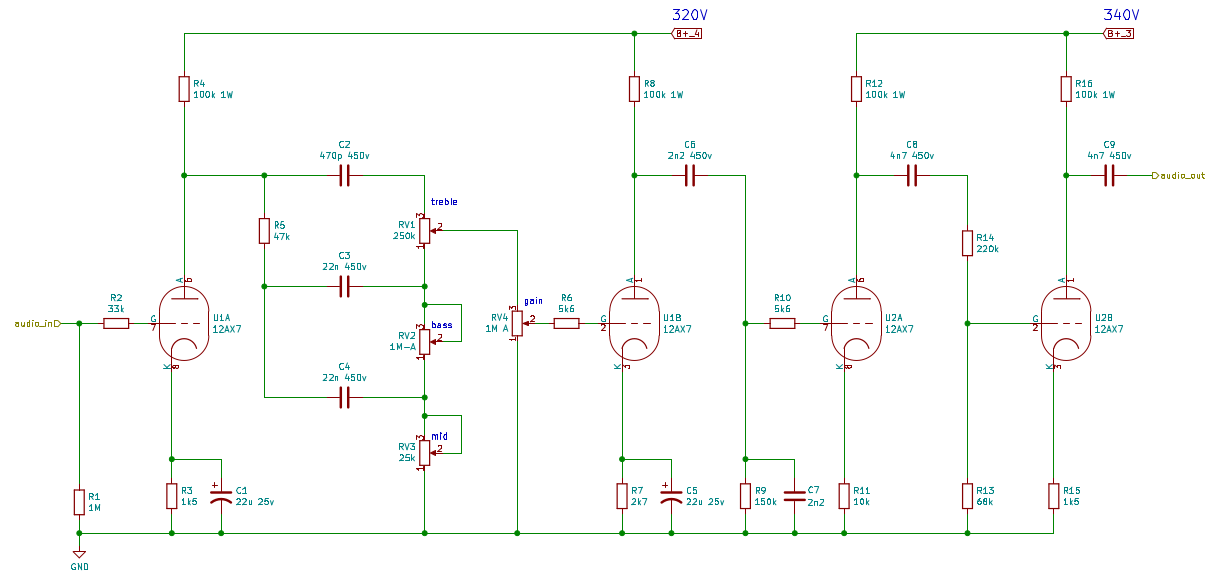
\includegraphics[width=\textwidth]{preamp_circuit.png}
\end{figure}

Notable features of this preamp are the tone shaping before the distortion, and small value coupling caps which shave bass frequencies. This circuit is pretty bright and ``cutting'', with enough gain for lots of preamp distortion. It can't quite do modern high-gain metal tones, but it does get pretty darn crunchy. It cleans up very well with the gain control set low, and using the volume control on your guitar is effective for doing the ``clean to mean'' thing. 

Both the clean and distorted tones sound great to me. It has lots of sustain and harmonic richness. It can tend towards overly bright and brittle tones, but adjusting the treble control, the tone pot on your guitar, and pick attack can mitigate this. The bright and cutting sounds can also help the guitar sit well in a mix.

\section{Power Amp}

The single 6550 output tube was chosen to provide a little more ``oomph'' than a typical Champ-style single ended amp, but still be fairly low power for playing at home or in the studio at reasonable volumes. I was looking for about 8 to 10 watts of clean output power, and about 15 watts when heavily overdriven.

\begin{figure}[H]
\centering
\caption{Power amp circuit}
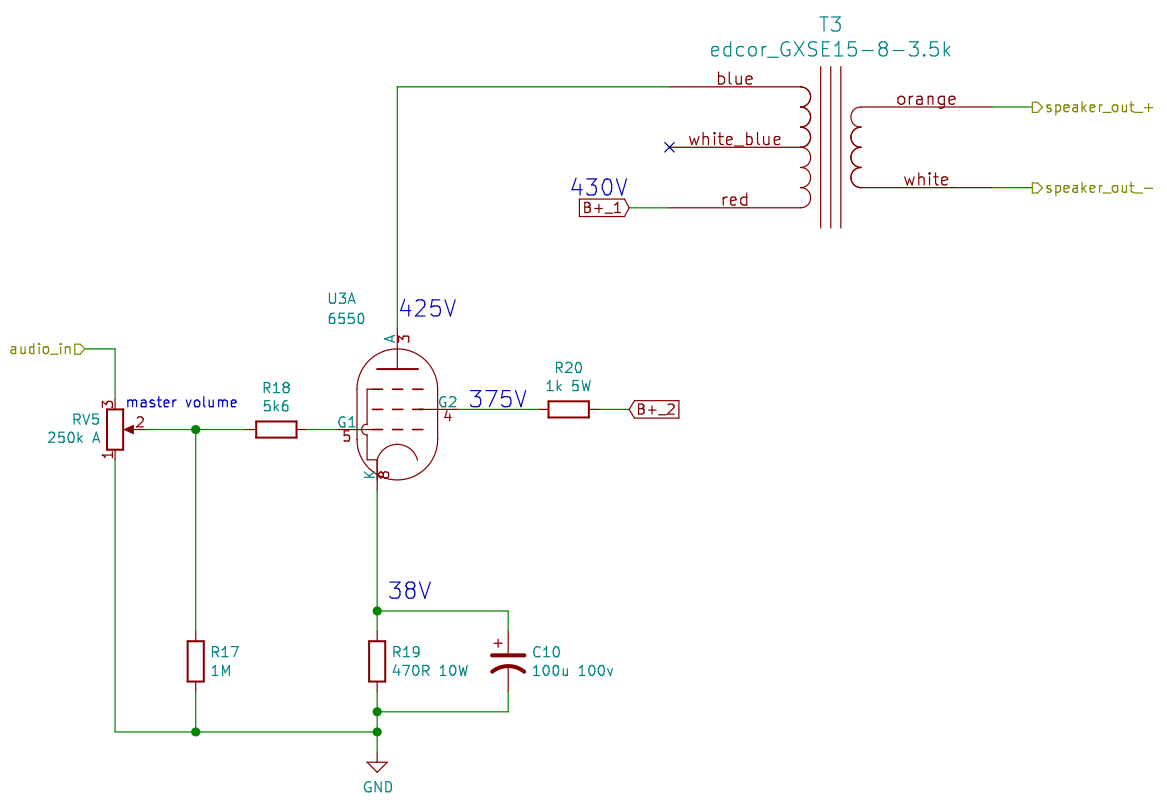
\includegraphics[width=\textwidth]{power_amp_circuit.png}
\end{figure}

As we can see by examining the voltage across the cathode resistor, about $80mA$ of bias current flows in the power tube at idle, for about 31 watts of dissipation. The maximum plate dissipation for this tube is 35 watts. I could probably bump up the bias current a little bit, there is no compelling reason to do so for now. 

Erring on the cold side will increase tube life and decrease heat in the chassis. Large output swings will be a little bit asymmetric and will introduce a little DC current in the output transformer, but the OT can handle it and a little asymmety sounds good for overdriven guitar sounds.

After construction, the amp was hooked up to a dummy load to test the power output. The output transformer has a 438:1 impedance ratio, and a variety of load resistances were tried out to experiment with the relationship between load impedance and power delivery. I have a big honkin' dummy load made up of a string of eight 2$\Omega$ resistors, and this allowed me to vary the load resistance, and thus the reflected primary impedance, by clipping heavy test leads across various resistors. The findings are summarized in the table below:

\begin{table}[H]
\centering
\begin{tabular}{ c | c | c }
    Load resistance  & Reflected impedance & Power out (Watts)  \\ \hline \hline
	4 & 1750 & 5.8 \\ \hline
	6 & 2628 & 8.5 \\ \hline
	8 & 3500 & 9.7 \\ \hline
	10 & 4380 & 10 \\ \hline
	12 & 5256 & 9.2 \\ \hline
	14 & 6132 & 8.8 \\ \hline
	16 & 7008 & 7.9 \\ \hline
\end{tabular}
\end{table}

The measured power output is an approximation and shouldn't be taken as a super precise measurement. I adjusted the signal to \textit{just} under the point of clipping while measuring the power output for each impedance, but this is a guitar amp and there is significant nonlinearity well below clipping. The exact point where ``clean signal'' stops and ``clipping'' begins is a soft and blurry line, but I tried to at least keep things reasonably consistent between readings. 

The above table shows us that somewhere around 3.5k to 5k is a happy primary impedance for this circuit if we want to get the most out of the setup as it is. The 3.5k$\Omega$ primary impedace from the output transformer I had lying around seems OK. With experimentation, we could tweak the B+ supply and the load to maximize power out, but a watt or two in either direction isn't going to make or break the amp.

The distortion introduced by overdriving the power amp is quite pleasant, with a gradual introduction of compression, then crunch, then heavy distortion. This is illustrated in the oscilloscope shots below:

\begin{figure}[H]
    \centering
    \subfloat[\centering]{{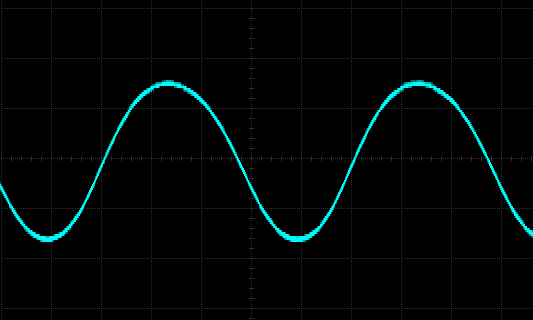
\includegraphics[width=.4\textwidth]{power_amp_scope_1.png} }}
    \qquad
    \subfloat[\centering]{{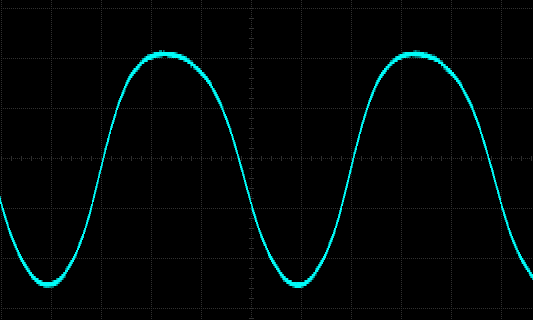
\includegraphics[width=.4\textwidth]{power_amp_scope_2.png} }}
    
    \subfloat[\centering]{{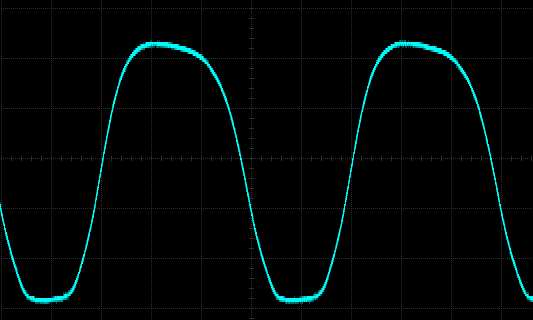
\includegraphics[width=.4\textwidth]{power_amp_scope_3.png} }}
    \qquad
    \subfloat[\centering]{{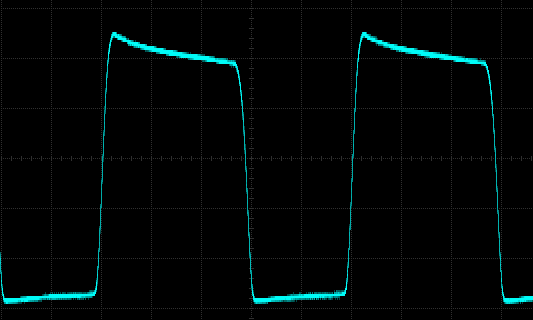
\includegraphics[width=.4\textwidth]{power_amp_scope_4.png} }}
\end{figure}

The asymmetric nature of the distortion is mostly due to the somewhat cold bias current. To me, the circuit sounds good and hits the desired output power, so there is little motivation to try to bring it right into the center of class A or squeeze every last clean milliwatt out of it.

The final output power delivered into an 8 $\Omega$ load is about 10 watts at ``somewhere below five percent'' distortion, and about 15 watts when hard clipping, right on target. I don't have the equipment to accurately measure distortion, so the clean output was ``eyeballed''. IMO, this is good enough for guitar work.

\section{Power supply}

The basic power supply plan is fairly standard, but the power transformer was scavanged from the bin so I had to futz around a little bit. The Hammond power transformer used only has a 115 volt primary winding. This caused all of the secondary voltages to come out a bit high when fed from a modern 120 volt wall outlet. 

To keep the B+ reasonable and, more importantly, to keep the heater voltage in spec, I used the 5 volt winding in ``bucking'' configuration  in series with the primary to reduce all secondary voltages a little bit. Modern Hammond transformers have improved the primary windings to be more compatible with modern wall voltages, but this trick was used so that I could use up an old dust bin transformer which was otherwise suitable.

\begin{figure}[H]
\centering
\caption{Main power supply}
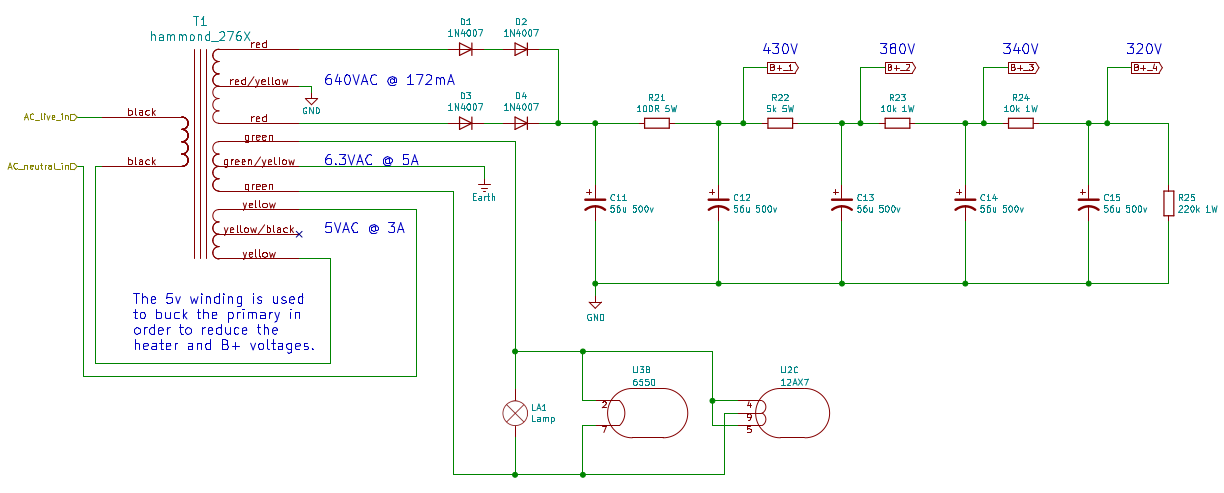
\includegraphics[width=\textwidth]{power_supply_1.png}
\end{figure}

After construction, the amp sounded pretty good and the noise performance was quite acceptable. But there was a small amount of 60/120Hz AC buzz coming from the first stage. Since there is so much gain in the preamp, a small amount of noise can become annoying when you crank the gain. I've heard much worse from popular amps, but since this is a hobby project I can afford to spend some effort improving the noise performance. To get things really quiet, I decided to use a DC heater supply for the first 12AX7 tube.

I initially tried to rectify the existing 6 volt winding and use the smoothed DC for just the first tube. This did improve the buzz coming from the first gain stage, but it worsened the buzz coming from the second preamp tube. This is a common problem when trying to do DC heaters as simply as possible, especially in a small chassis. The rectification causes the existing AC supply to become more distorted, and high frequency components are injected into the signal path.

To get things really quiet, I added a small transformer to create a DC heater supply just for V1. I used a small 15 volt transformer that I had kicking around for this. The 15 volts AC is fed into a bridge rectifier, then smoothed with a large capacitor, then fed into an RC filter wich provides further ripple reduction and drops the voltage to right around 12.6 volts DC when loaded with a single 12AX7 heater wired for 12 volt operation.

\begin{figure}[H]
\centering
\caption{DC heater supply for V1}
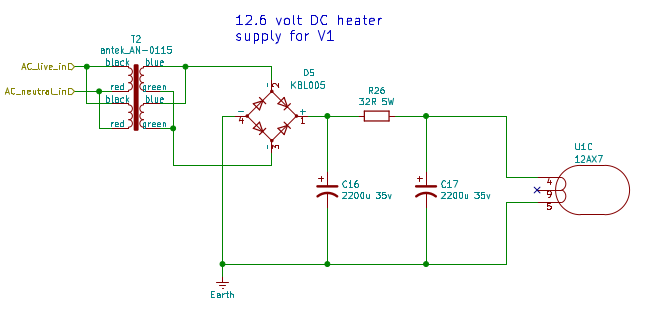
\includegraphics[width=\textwidth]{power_supply_2.png}
\end{figure}

With the first tube heater supplied by this smooth DC voltage generated from a different widing than the rest of the 6 volt AC heaters, the amp has very good noise performance. There is some white-noise-ish hiss and a very small amount of power line frequency buzz when the gain control and master volume are both set very high, but this is to be expected in any high gain tube circuit. Most importantly to me, the noise is dominated by hiss, with very low levels of 60 Hz related hum and buzz.

\section{Construction}

The amp was built in the carcass of a Fender Vibro-Champ XD amp that a local guitar store was throwing away. I stripped everything out of the chassis and drilled most of the threaded standoffs out.

The circuit is all point-to-point construction using terminal strips. The tubes are layed out so that the signal path is very straghtforward and signal wires don't meander all over the chassis. Noisy rectifiers and heaters are kept far from sensitive audio nodes.

\begin{figure}[H]
\centering
\caption{Guts}
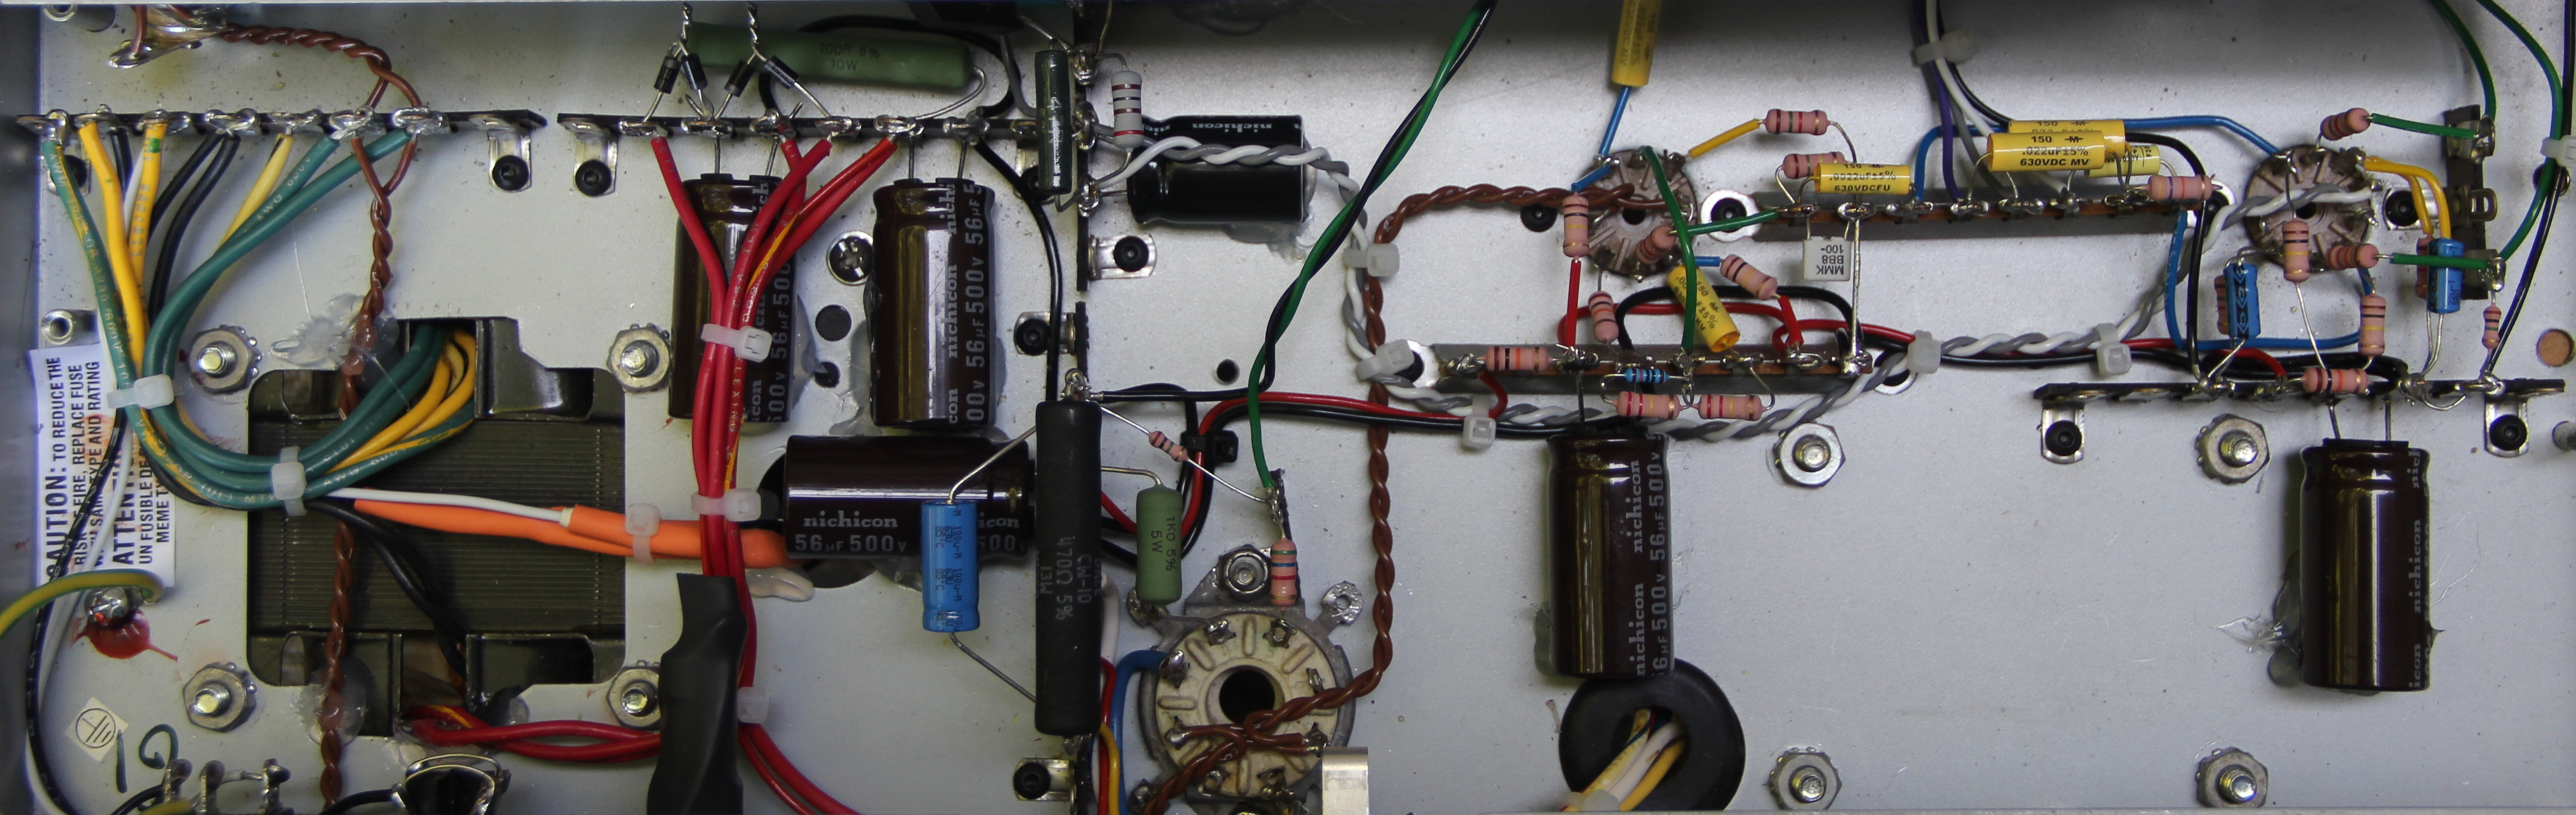
\includegraphics[width=\textwidth]{guts.jpg}
\end{figure}

The chassis does get quite hot. The 6550 power tube is dissipating around 30 watts, and its heat rises straight up into the chassis. There are a handful more watts inside the chassis, mostly in the cathode bias resistor for the power tube and the dropping resistor for the DC heater supply.

This is a tube amp though, so hot and toasty is to be expected. None of the components are overly stressed, and reliablility should be quite good. Due to the point-to-point construction, repairs and mods are somewhat annoying to perform, but infinitely possible.

The original Fender donor combo amp came with an 8" speaker, which is just too small for serious guitar sounds at all but the lowest volumes. Additionally, the baffle was made of really cheesy particle board. I made a new baffle out of decent 1/2" plywood with a cutout for a 10" speaker and reapplied the old grill cloth. The Warehouse Vet-10 10" speaker \textit{juuuuuust} fits, other speakers may or may not fit at all. 

The power tube is very close to the magnet, and the spring tube retainer I installed occasionally rattles sympathetically at loud volumes. This is not a major problem, I'll leave it for now and reasses if it becomes annoying later.

\section{Conclusion}

This prototype is a definte success. The noise performance is very good and the power output is right where I wanted it to be. The sound is very nice. There is a range of sparkly cleans, crunchy, and fuzzy sounds in there. The prototype would be perform very well as a practice amp at home, and would probably record pretty well.

The limiting factor is mainly the lame tiny MDF cabinet. Repurposing the dead Fender combo was economical, but a slightly larger cabinet made of better materials would be an improvement. The amp would be pretty at home in a Princeton sized cabinet if another one is made. This would allow for trying out different 10" speakers without worrying about the magnet coming into contact with the power tube.

The next step would be to build another version with selected, instead of stumbled upon, parts. I've layed out a pcb for the preamp and chosen some transformers that I think will work. Unfortunately this will probably be on hold for a while, as the semester is starting up and I won't have much time for fun hobbies until winter break.

\section{About the Name}

When I used to repair tube amplifiers, it was common for the various ``Champs'' to come through the shop for servicing. There is the Fender Champ, the Champion, the Vibro-Champ, the Super-Champ, the list goes on. Whenever I had one of these on my bench, I would always sing to it:

\begin{poem}
\begin{stanza}
You are the Champion\verseline
My frie-end\verseline
And you'll keep on fighting\verseline
Til the end\end{stanza}

\begin{stanza}
You are the Champion\verseline
You are the Champion\verseline
No time for losers\verseline
Cause you are the Champion\end{stanza}
... etc
\end{poem}

Since this amp roughly occupies ``Champ'' territory, only with more output power and with a much meatier preamp, naturally \textbf{It is the Champion}.

\end{document}